\documentclass[runningheads]{llncs}

\usepackage[T1]{fontenc}
\usepackage{graphicx}
\usepackage{booktabs}
\usepackage{multirow}
\usepackage{amsmath}
\usepackage{cite}
\usepackage{float}

\begin{document}
\sloppy
\title{Generating Blood Cells with Machine Learning}

\author{Débora Sofia Valério Taborda de Seiça} % chktex 8
%
\authorrunning{D. Seiça}
% First names are abbreviated in the running head.
% If there are more than two authors, 'et al.' is used.

\institute{University of Coimbra, Portugal \\
\email{uc2018278107@student.uc.pt}}

\maketitle% typeset the header of the contribution

\section{Introduction}

Image Quality Assessment (IQA) plays a critical role in domains such as biometric authentication, multimedia processing, and medical imaging~\cite{kim2015face, huang2020facerecon}. It broadly refers to the estimation of visual quality based on attributes like contrast, sharpness, noise, and the presence of artifacts. Within this domain, Facial Image Quality Assessment (FIQA) focuses specifically on facial images, where quality is not assessed in terms of visual aesthetics, but rather in terms of its impact on the performance of face recognition systems~\cite{cavazos2021racebias, terhoerst2020demobias}.

IQA methods fall into two categories: subjective and objective. Subjective methods use human ratings to measure perceived quality, often summarized as Mean Opinion Scores (MOS)~\cite{ITU-R-BT500}. These scores are reliable but expensive to collect and not scalable. Objective methods rely on algorithms to estimate quality, either by comparing to a reference image or by analyzing features of the image itself.

Objective methods can be divided into full-reference (FR) and no-reference (NR). FR methods compare a distorted image to a clean reference. They are often accurate but can only be used when a reference is available. NR methods estimate quality without a reference and are more practical in real-world settings, though they often struggle to generalize across distortions and content~\cite{shahrukh2019survey}.

FIQA is a subdomain of IQA focused on facial images. It plays a key role in biometric applications such as identity verification, where reference images are typically unavailable, and is also relevant in non-biometric scenarios like surveillance and forensic analysis. Consequently, most FIQA methods are no-reference NR, relying on task-specific priors or learned representations to estimate image quality~\cite{hernandez2019faceqnet}.

A key challenge in IQA is the gap between objective metrics and human perception. Classical metrics such as PSNR~\cite{gonzalez2002digital} (Peak Signal-to-Noise Ratio), SSIM~\cite{wang2004ssim} (Structural Similarity Index), and VIF~\cite{sheikh2006image} (Visual Information Fidelity) provide automatic quality estimates but often show weak correlation with human ratings across datasets~\cite{shahrukh2019survey}. This issue is more pronounced in facial images, where perceived quality is shaped by both image distortions and biases from the observer.

Studies have shown that FIQA is affected by both demographic and non-demographic biases. Perceived quality can vary with ethnicity, gender, or age, often due to dataset imbalance and observer subjectivity~\cite{cavazos2021racebias, terhoerst2020demobias, kabbani2024demo}. For example, darker skin tones tend to produce lower recognition accuracy, and female faces are often rated with lower quality scores~\cite{huang2020facerecon}. These effects highlight the need for more inclusive and perceptually aligned quality metrics.

The International Civil Aviation Organization~\cite{icao-2015} (ICAO) and the International Organization for Standardization (ISO) and the International Electrotechnical Commission (IEC) 19794--5 standard~\cite{iso-iec29794-5-2010} establish guidelines for image quality in Machine-Readable Travel Documents (MRTDs). These guidelines ensure uniform image conditions (e.g., lighting, focus, and resolution) and consistency across datasets. While these regulations establish a technical baseline, they do not account for perceptual biases and demographic variability in FIQA.\@

These biases raise ethical concerns. Legal frameworks, such as the European Convention on Human Rights (Article 14)~\cite{echr-article14}, the Universal Declaration of Human Rights (Article 7)~\cite{udhr-article7}, the General Data Protection Regulation (Article 22)~\cite{gdpr-article22}, the European Artificial Intelligence Act (2024)~\cite{eu-ai-act-2024} and the United States Bill of Rights~\cite{us-ai-bill-rights-2022}, aim to prevent discriminatory decisions. Still, biases persist, often introduced through human observers involved in labeling.

Neuroscience shows that face perception relies on the fusiform face area, a brain region specialized for facial stimuli~\cite{kanwisher2006fusiform, tsao2008mechanisms}. This biological specialization makes FIQA particularly sensitive to both stimulus features (e.g., age, gender, ethnicity, attractiveness) and the demographic background of the observers.

Steganographically distorted facial images pose a harder problem. Steganography hides data by slightly changing pixel values, often in ways that escape human detection~\cite{steganography}. Recent printed-proof techniques go further by ensuring that hidden data can survive physical printing and scanning noises, making them useful for secure document encoding. While these changes are visually minimal, they can damage biometric features and reduce recognition accuracy~\cite{stegastamp2020, codeface2021, stampone2024, riemannian2023}. NR methods are usually not designed to catch these small but critical degradations.

To handle these limitations, we propose a FIQA framework based on pseudo-MOS.\@ We first use a small set of facial images labeled with overall quality scores to train a fusion model that combines FR metrics into a single predictor. This model generates pseudo-MOS for the rest of the dataset. Using these labels, we then train a NR deep regressor based on a ResNet-18~\cite{resnet} pretrained on ImageNet~\cite{imagenet}, allowing it to estimate perceptual quality without needing a reference image.

Our approach bridges the gap between FR supervision and NR inference. It offers a scalable solution for evaluating images with subtle distortions, like steganography, and supports the development of quality assessment models tailored to domain-specific tasks. In doing so, it combines the accuracy of FR metrics with the practicality of NR models in a single IQA pipeline.

\section{Problem Statement}

The primary objective of this study is to implement, train, and comparatively evaluate three prominent generative model classes: GANs, VAEs, and Diffusion Models. We assess their effectiveness quantitatively by computing the Fréchet Inception Distance (FID)~\cite{heusel2017gans}, a robust metric to measure the similarity between generated and real image distributions. Additionally, we discuss qualitative results to highlight each model's strengths and limitations. The ultimate goal is to identify an optimal generative framework capable of producing realistic and diverse synthetic blood cell images.
\section{Approach}

We implemented and evaluated three classes of generative models. Each model was adapted to generate 28$\times$28 RGB images that resemble the blood cell samples in the BloodMNIST dataset.

For each approach, the model was trained on the entire dataset, combining the original training, validation, and test splits. All images were normalized to the $[-1, 1]$ range. We maintained a batch size of 128 and used the Adam optimizer for all models. Each training was repeated with five random seeds for later evaluation stability.

\textbf{VAE:} The Variational Autoencoder consists of a convolutional encoder that maps the input image into a latent Gaussian distribution, and a decoder that reconstructs the image from sampled latent vectors. The model is trained using a reconstruction loss combined with a Kullback-Leibler divergence term to regularize the latent space~\cite{kingma2013auto}.

\textbf{GAN:} We implemented a Deep Convolutional GAN (DCGAN), with a generator that learns to synthesize realistic images from latent noise vectors, and a discriminator that learns to distinguish between real and generated samples~\cite{goodfellow2014generative}. Both networks use strided convolutions and LeakyReLU activations. The generator is trained to fool the discriminator, while the discriminator is trained to correctly classify real and fake inputs.

\textbf{Diffusion:} The DDPM is a generative model based on a Markovian process that gradually adds noise to images and then learns to reverse this corruption step by step~\cite{ho2020denoising}. The training objective is to predict the added noise at each timestep, enabling the model to sample clean images from pure noise.

To ensure fairness, all models were trained using the same hardware environment and epochs, and evaluated using the Fréchet Inception Distance (FID) as a common metric.
\section{Experimental Setup and Evaluation}

To assess the effectiveness of the proposed method, we conduct qualitative and quantitative evaluations of the generated images.

\subsection{Experimental Setup}

We generate a dataset of augmented icons using a diverse set of textures from \texttt{texture\_pack}. The visibility factor $\alpha$ is varied within the predefined range, and random border expansions are applied. The output images are analyzed for their blending quality and degradation realism.

To ensure a fair evaluation, we consider multiple test cases with different texture types, including smooth, rough, and highly creased surfaces. Additionally, we vary the positioning of the icons to test the robustness of the algorithm against different spatial placements.

\subsection{Qualitative Evaluation}

Sample images generated using the proposed algorithm are visually examined to assess their consistency with real-world degradation effects. As shown in Figure~, the blended icons exhibit natural variations in contrast, smudging, and background integration. The images are compared with real-world printed and degraded icons to validate their visual authenticity.

Furthermore, we analyze how different textures impact the final blended output. Icons placed on highly wrinkled textures show more severe degradation, whereas smoother textures yield more subtle blending effects. These qualitative insights help refine the augmentation process.

\subsection{Quantitative Evaluation}

To quantify the effectiveness of the blending, we compute similarity metrics such as the Structural Similarity Index (SSIM) and Peak Signal-to-Noise Ratio (PSNR) between the augmented icons and real-world degraded icons. Higher SSIM values indicate a closer resemblance to naturally degraded images, while PSNR provides an objective measure of signal distortion.

Additionally, we perform a perceptual evaluation by conducting a user study where participants rate the realism of the generated images on a Likert scale. The user study includes a diverse group of individuals who assess whether the augmented images convincingly mimic real-world degradation. Statistical analysis of the responses provides insights into the subjective quality of the augmentation technique.

\subsection{Results and Discussion}

The evaluation results demonstrate that the proposed method produces highly realistic degraded icons with minimal artifacts. The combination of texture-based blending and height-map-driven degradation ensures that the output images closely resemble real-world printed icons exposed to wear and environmental effects.

Table~ presents a summary of the SSIM and PSNR values for different texture categories. The results indicate that textures with higher roughness lead to lower SSIM scores, which aligns with the expectation that increased degradation reduces structural similarity. However, user study results suggest that these variations contribute positively to the perceived authenticity of the degradation effects.

The findings highlight the strengths of the proposed method in generating realistic augmentations while also identifying areas for further improvement, such as fine-tuning degradation intensity based on specific use cases.

\section{Results and Analysis}

Table~\ref{tab:fid-scores} summarizes the mean and standard deviation of the FID scores obtained for each model across five independent runs.

\begin{table}[h]
\centering
\caption{Fréchet Inception Distance (FID) results over 5 runs. Lower is better.}\label{tab:fid-scores}
\begin{tabular}{lcc}
\toprule
\textbf{Model} & \textbf{Mean} & \textbf{Std. Dev.} \\
\midrule
VAE        & 201.73 & 0.23 \\
GAN        & 180.57 & 0.71 \\
Diffusion  & 423.70 & 0.64 \\
\bottomrule
\end{tabular}
\end{table}

\begin{figure}
    \centering

    \begin{minipage}[t]{0.48\textwidth}
        \centering
        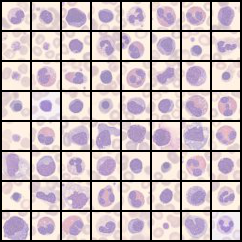
\includegraphics[width=\linewidth]{images/real.png}
        (a) Real Images
    \end{minipage}
    \hfill
    \begin{minipage}[t]{0.48\textwidth}
        \centering
        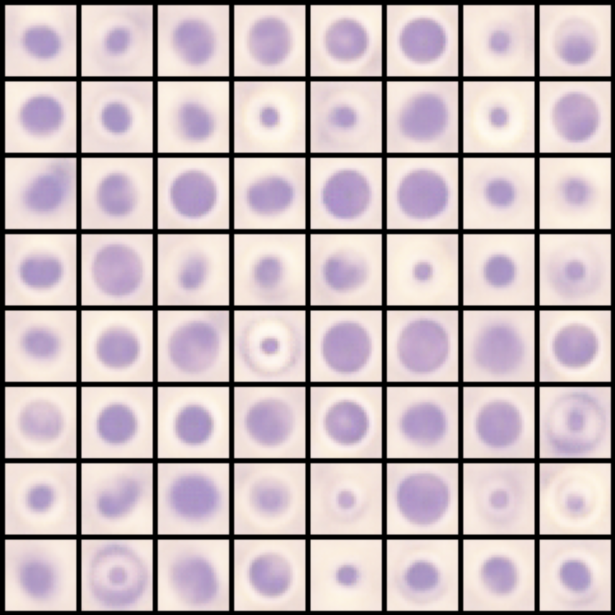
\includegraphics[width=\linewidth]{images/vae.png}
        (b) VAE Samples
    \end{minipage}

    \vspace{0.5em}

    \begin{minipage}[t]{0.48\textwidth}
        \centering
        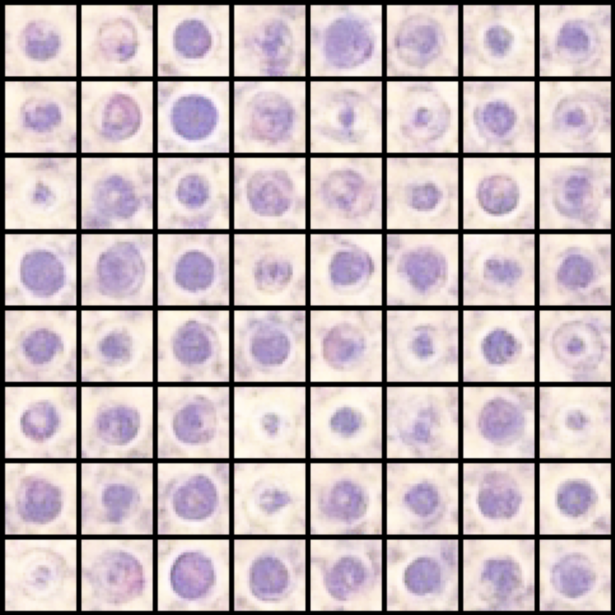
\includegraphics[width=\linewidth]{images/gan.png}
        (c) GAN Samples
    \end{minipage}
    \hfill
    \begin{minipage}[t]{0.48\textwidth}
        \centering
        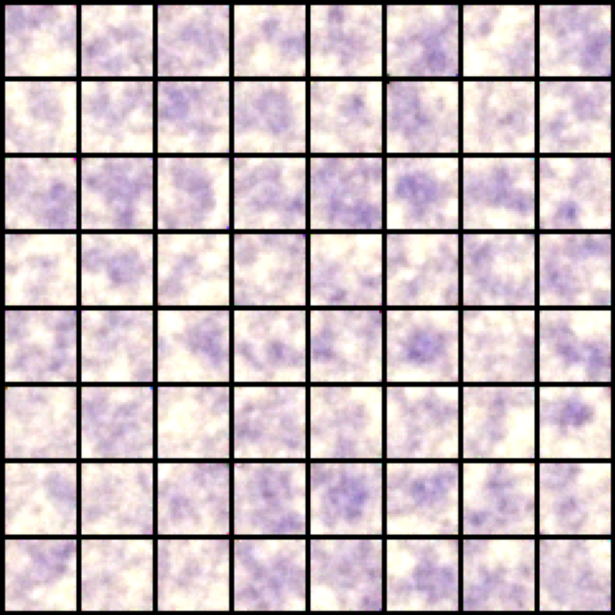
\includegraphics[width=\linewidth]{images/diffusion.png}
        (d) Diffusion Samples
    \end{minipage}

    \caption{Qualitative comparison of real and generated blood cell images.}\label{fig:model-comparison}
\end{figure}

Figure~\ref{fig:model-comparison} shows both the real images and the visual samples generated by each model. The results reveal clear qualitative differences. The VAE samples exhibit smooth but often blurry outputs due to its probabilistic reconstruction objective. Diffusion models produce a lump of blobs, barely resembling a blood cell. GANs generate highly detailed and diverse samples, closely resembling real blood cells.

Overall, GANs achieve the best quantitative and qualitative performance, indicating superior capability in modeling complex visual structures present in biomedical data.

\section{Conclusion}

In this study, we implemented and evaluated three prominent classes of generative models, Variational Autoencoders (VAEs), Generative Adversarial Networks (GANs), and Denoising Diffusion Probabilistic Models (DDPMs), on the BloodMNIST dataset. Each model was trained under consistent conditions and assessed using both qualitative visualizations and the Fréchet Inception Distance (FID) metric.

The results revealed clear differences in performance. The VAE produced smooth but blurry reconstructions due to its probabilistic decoder. Diffusion models failed to produce visually coherent images, resulting in noisy outputs that barely resemble blood cells. In contrast, GANs achieved the best visual quality, generating diverse and realistic samples that closely match real data.

These observations align with the FID scores reported in Table~\ref{tab:fid-scores}, where GANs obtained the lowest value (180.57), outperforming both VAEs (201.73) and diffusion models (423.70). This demonstrates the effectiveness of adversarial training for modeling complex biomedical structures.

Overall, GANs offer the best balance of fidelity and diversity for blood cell image synthesis in this context. Future work may explore hybrid or conditional architectures to further improve control over generated samples and class specificity.


\bibliographystyle{splncs04}
\bibliography{references}

\end{document}
